\section{Application and Comparison}
This chapter covers the application of random forest regression and the evaluation of its performance.

In section \ref{sec:simulation}, we apply the random forest on simulated data, 
and show how its performance develops over increasing sample sizes.

Then in section \ref{sec:real_data}, we apply the random forest on the real Titanic data set \cite{titanicData}
and evaluate its performance.

In section \ref{sec:adaboost} and \ref{sec:gradient_boosting}, we apply AdaBoost and Gradient
Boosting respectively on the Titanic data set and  compare their performance with that of the random forest.

\subsection{Application of Random Forest on simulated data}
\label{sec:simulation}

In the simulation, we use a linear and a non-linear data generating process (DGP) for random forest regression.
The linear DGP generates the data tuples \( (y, x_{1}, x_{2}, x_{3}) \) as follows:

\begin{equation}\label{eq:linear_dgp}
    y = \beta_{0} + \beta_{1} x_{1} + \beta_{2} x_{2} + \beta_{3} x_{3} + \epsilon,
\end{equation}

whereas \( (\beta_{0}, \beta_{1}, \beta_{2}, \beta_{3}) = (0.3, 5, 10, 15) \),
\( x_{1}, x_{2}, x_{3} \sim \mathcal{N}(0,\,3) \), and \( \epsilon \sim \mathcal{N}(0,\,1) \).

The performance of the Random Forest over an increasing sample is illustrated
below in figure \ref{fig:forest_vs_ols_linearDGP} and \ref{fig:forest_vs_ols_nonLinearDGP}.
For each sample drawn from the linear DGP, a set of parameters
were optimized via cross validation. Then, the residual sum of squares (RSS) gets calculated
based on the holdout set of 100 instances.

\begin{figure}
    \captionsetup{format=plain}
    \makebox[\textwidth]{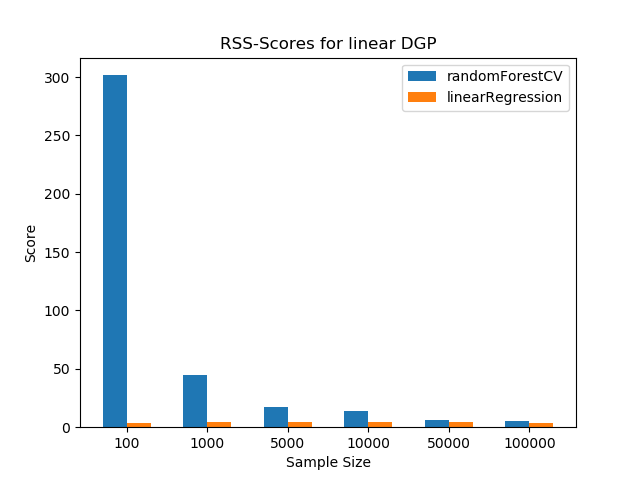
\includegraphics[width=120mm]{forest_vs_ols_linearDGP.png}}
    \caption
        {This plot illustrates the RSS for different training sample sizes for Random Forest and OLS.
        These samples where drawn from a linear DGP in accordance to equation (\ref{eq:linear_dgp}).
        The holdout set for calculating the RSS were drawn again for each training sample from the same DGP.
        It always contained 100 observations. In case of the Random Forest, for each sample the parameters
        got optimized again via cross validation.
        }
    \label{fig:forest_vs_ols_linearDGP}
\end{figure}

As one can see in figure \ref{fig:forest_vs_ols_linearDGP}, the RSS of the Random Forest converges for the linear DGP
to that of the OLS for increasing sample sizes. 

The non-linear DGP generates the data tuples \( (y, x_{1}, x_{2}) \) as follows:

\begin{equation}\label{eq:non_linear_dgp}
    y = \beta_{0} + \beta_{1} I(x_{1} >= 0, x_{2} >= 0) + \beta_{2} I(x_{1} >= 0, x_{2} < 0) + \beta_{3} I(x_{1} < 0) + \epsilon,
\end{equation}

whereas \( (\beta_{0}, \beta_{1}, \beta_{2}, \beta_{3}) \), \( x_{1}, x_{2} \) and \(  \epsilon \)
are the same in the previous DGP.

\begin{figure}[H]
    \captionsetup{format=plain}
    \makebox[\textwidth]{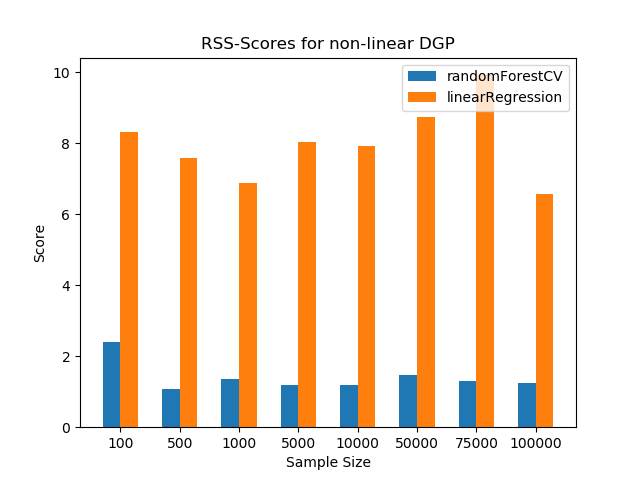
\includegraphics[width=120mm]{forest_vs_ols_nonlinearDGP.png}}
    \caption
        {This plot illustrates the RSS for different training sample sizes for Random Forest and OLS.
        These samples where drawn from a non-linear DGP in accordance to equation (\ref{eq:non_linear_dgp}).
        The holdout set for calculating the RSS were drawn again for each training sample from the same DGP.
        It always contained 100 observations. In case of the Random Forest, for each sample the parameters
        got optimized again via cross validation.
        }
    \label{fig:forest_vs_ols_nonLinearDGP}
\end{figure}

As one can see above in figure \ref{fig:forest_vs_ols_nonLinearDGP}, the Random Forest performs strictly better
than the OLS for any sample size. Due to this DGP resembling a stratification similar to
that of a Descision Tree, the RSS of the Random Forest converges relatively quickly while that of the OLS
remains unstable and high. 